% !TEX root =  ../main_manuscript.tex 
\subsection{Statistical Model}
For developing an upgrading-risk prediction model, the available data in the PRIAS cohort was patient age at inclusion in AS, longitudinally measured PSA, timing of repeat biopsies and corresponding Gleason grades, and observed time of upgrading. Analysis of this data required modeling the within-patient correlation for PSA, the association between the Gleason grades and PSA profiles of a patient, and handling missing PSA measurements after a patient experienced upgrading. In such situations, a commonly used model is the joint model for time-to-event and longitudinal data~\citep{tomer2019,coley2017prediction,rizopoulos2012joint}.

Our joint model consisted of two sub-models. First, a linear mixed sub-model~\citep{laird1982random} for longitudinally measured PSA (log-transformed). Second, a relative-risk sub-model (similar to the Cox model) for obtaining the cause-specific upgrading-risk. Patient age was included as a predictor in both sub-models. In the PSA sub-model, we fitted a curve to the PSA measurements (Panel~A, Figure~\ref{fig:jmExplanationPlot_113}). Subsequently, we calculate the mathematical derivative of the fitted PSA profile over time to obtain PSA velocity. This instantaneous velocity is flexible over follow-up (Panel~B, Figure~\ref{fig:jmExplanationPlot_113}), and hence captures more information than the widely employed constant PSA velocity~\citep{vickers2009psavelocity}. We modeled the impact of PSA on upgrading-risk by including fitted PSA value and velocity as predictors in the relative-risk model. Also, the time of the latest negative biopsy was utilized in the relative-risk sub-model (Panel~C, Figure~\ref{fig:jmExplanationPlot_113}). The parameters of the two sub-models were estimated jointly (Supplementary~A) using the R package \textbf{JMbayes}~\citep{rizopoulosJMbayes}. 

\begin{figure}
\centerline{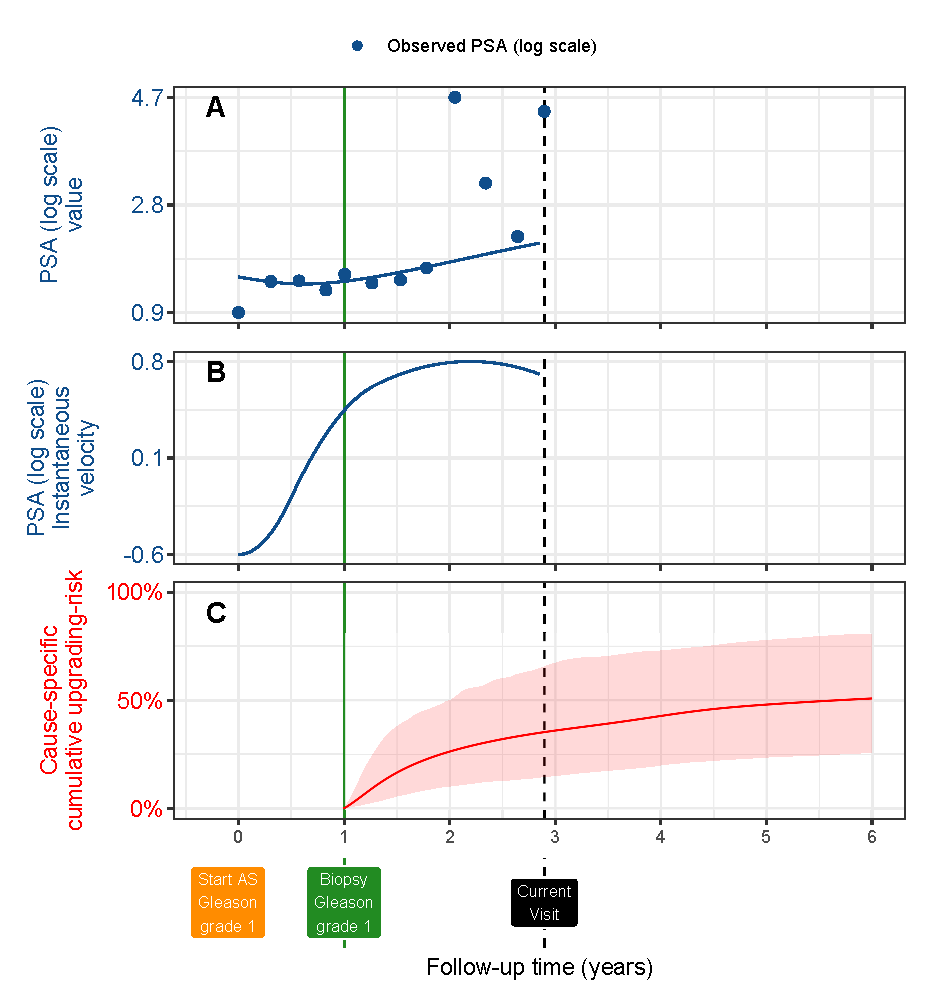
\includegraphics[width=\columnwidth]{images/jmExplanationPlot_113.eps}}
\caption{\textbf{Illustration of the joint model on a real PRIAS patient}. \textbf{Panel~A:} Observed PSA (blue dots) and fitted PSA (solid blue line), log-transformed. \textbf{Panel~B:} Estimated instantaneous velocity of PSA (log-transformed). \textbf{Panel~C}: Predicted cause-specific cumulative upgrading-risk (95\% credible interval shaded). Upgrading is defined as an increase in the Gleason grade group from group~1~\citep{epsteinGG2014} to 2 or higher. This upgrading-risk is calculated starting from the time of the latest negative biopsy (vertical green line at year 1 of follow-up). The joint model estimated it by combining the fitted PSA (log scale) value and instantaneous velocity, and time of the latest negative biopsy. Black dashed line at year 3 denotes the time of current visit.}
\label{fig:jmExplanationPlot_113}
\end{figure}

\subsection{Model Validation}
We validated our PRIAS based risk prediction model internally in the PRIAS cohort, and externally using the largest five GAP3 database cohorts (Section~\ref{subsec:cohort} and Supplementary~A.2). We assessed our model's ability to discriminate between patients who experience/do not experience upgrading via the area under the receiver operating characteristic curve or AUC~\citep{rizopoulos2017dynamic}. We employed calibration plots~\citep{royston2013external,steyerberg2010assessing} and mean absolute risk prediction error~\citep{rizopoulos2017dynamic} to graphically and quantitatively evaluate our model's risk prediction accuracy. Since AS studies are longitudinal, both AUC and prediction error vary over follow-up (Supplementary~B.1). Lastly, to resolve any potential model miscalibration in validation cohorts, we aimed to recalibrate our model's baseline hazard of upgrading (Supplementary~A), individually for each cohort.